\documentclass{article}

\usepackage[letterpaper, portrait, margin=1.5in]{geometry}

\usepackage{fancyhdr}
\usepackage{ragged2e}
\usepackage{graphicx}
\usepackage{caption}
\usepackage{amsmath}
\usepackage{rotating}

\usepackage{listings}
\usepackage{color}

\definecolor{dkgreen}{rgb}{0,0.6,0}
\definecolor{gray}{rgb}{0.5,0.5,0.5}
\definecolor{mauve}{rgb}{0.58,0,0.82}

\lstset{frame=tb,
  language=Java,
  aboveskip=3mm,
  belowskip=3mm,
  showstringspaces=false,
  columns=flexible,
  basicstyle={\small\ttfamily},
  numbers=none,
  numberstyle=\tiny\color{gray},
  keywordstyle=\color{blue},
  commentstyle=\color{dkgreen},
  stringstyle=\color{mauve},
  breaklines=true,
  breakatwhitespace=true,
  tabsize=4
}

\setcounter{secnumdepth}{1}

\usepackage{chngcntr}
\counterwithin{figure}{section}

\renewcommand*{\thepage}{C\arabic{page}}

\pagestyle{fancy}
\lhead{ACME Robotics}
\chead{\#8367}
\rhead{\ifcontents Contents \else Week \thesection \fi}

\newif\ifcontents
\contentstrue

\makeatletter
\renewcommand{\@seccntformat}[1]{}
\makeatother
\begin{document}

\subsection{Lift 2.0 Fabrication}
%! entry
Early in this week, Oren went to meet with the local welder to begin the process of setting up and welding both the box frame and the carriage for the new lift. He was hoping to complete the new lift by Tuesday, as to give the drivers enough time to practice, but unfortunately hit some complications and the lift wasn't completed in time. So Oren focused the rest of his time making sure the current lift was running as well as possible. Which required him to deconstruct the lift, sand down rough spots on the runners and change out broken bearing to allow for the lift to run. After which he assembled everything and bolted it back onto the robot ready for Norcals. 

\subsection{Attaching a Second Pull Up Run}
Another problem that had been pointed out after the Napa tournament was that the lift would tilt when at max height because of only having the one pull up run. To fix this, another pull up run was needed to be created. Ashlin and Aidan had already made extra bearing standoffs that could work for the new pull up run. The only problem was that the wire run up sheath was placed right where the new pull up run needed to be. Oren fixed this by placing a piece of aluminum that ran upwards for the wire sheath but was offset for the left by a few inches as shown in Figure \ref{fig:PullUp}. This solution worked and the wires didn't get in the way. The second pull up run allowed the lift to maximize height without tilting.

\begin{figure}
    \centering
    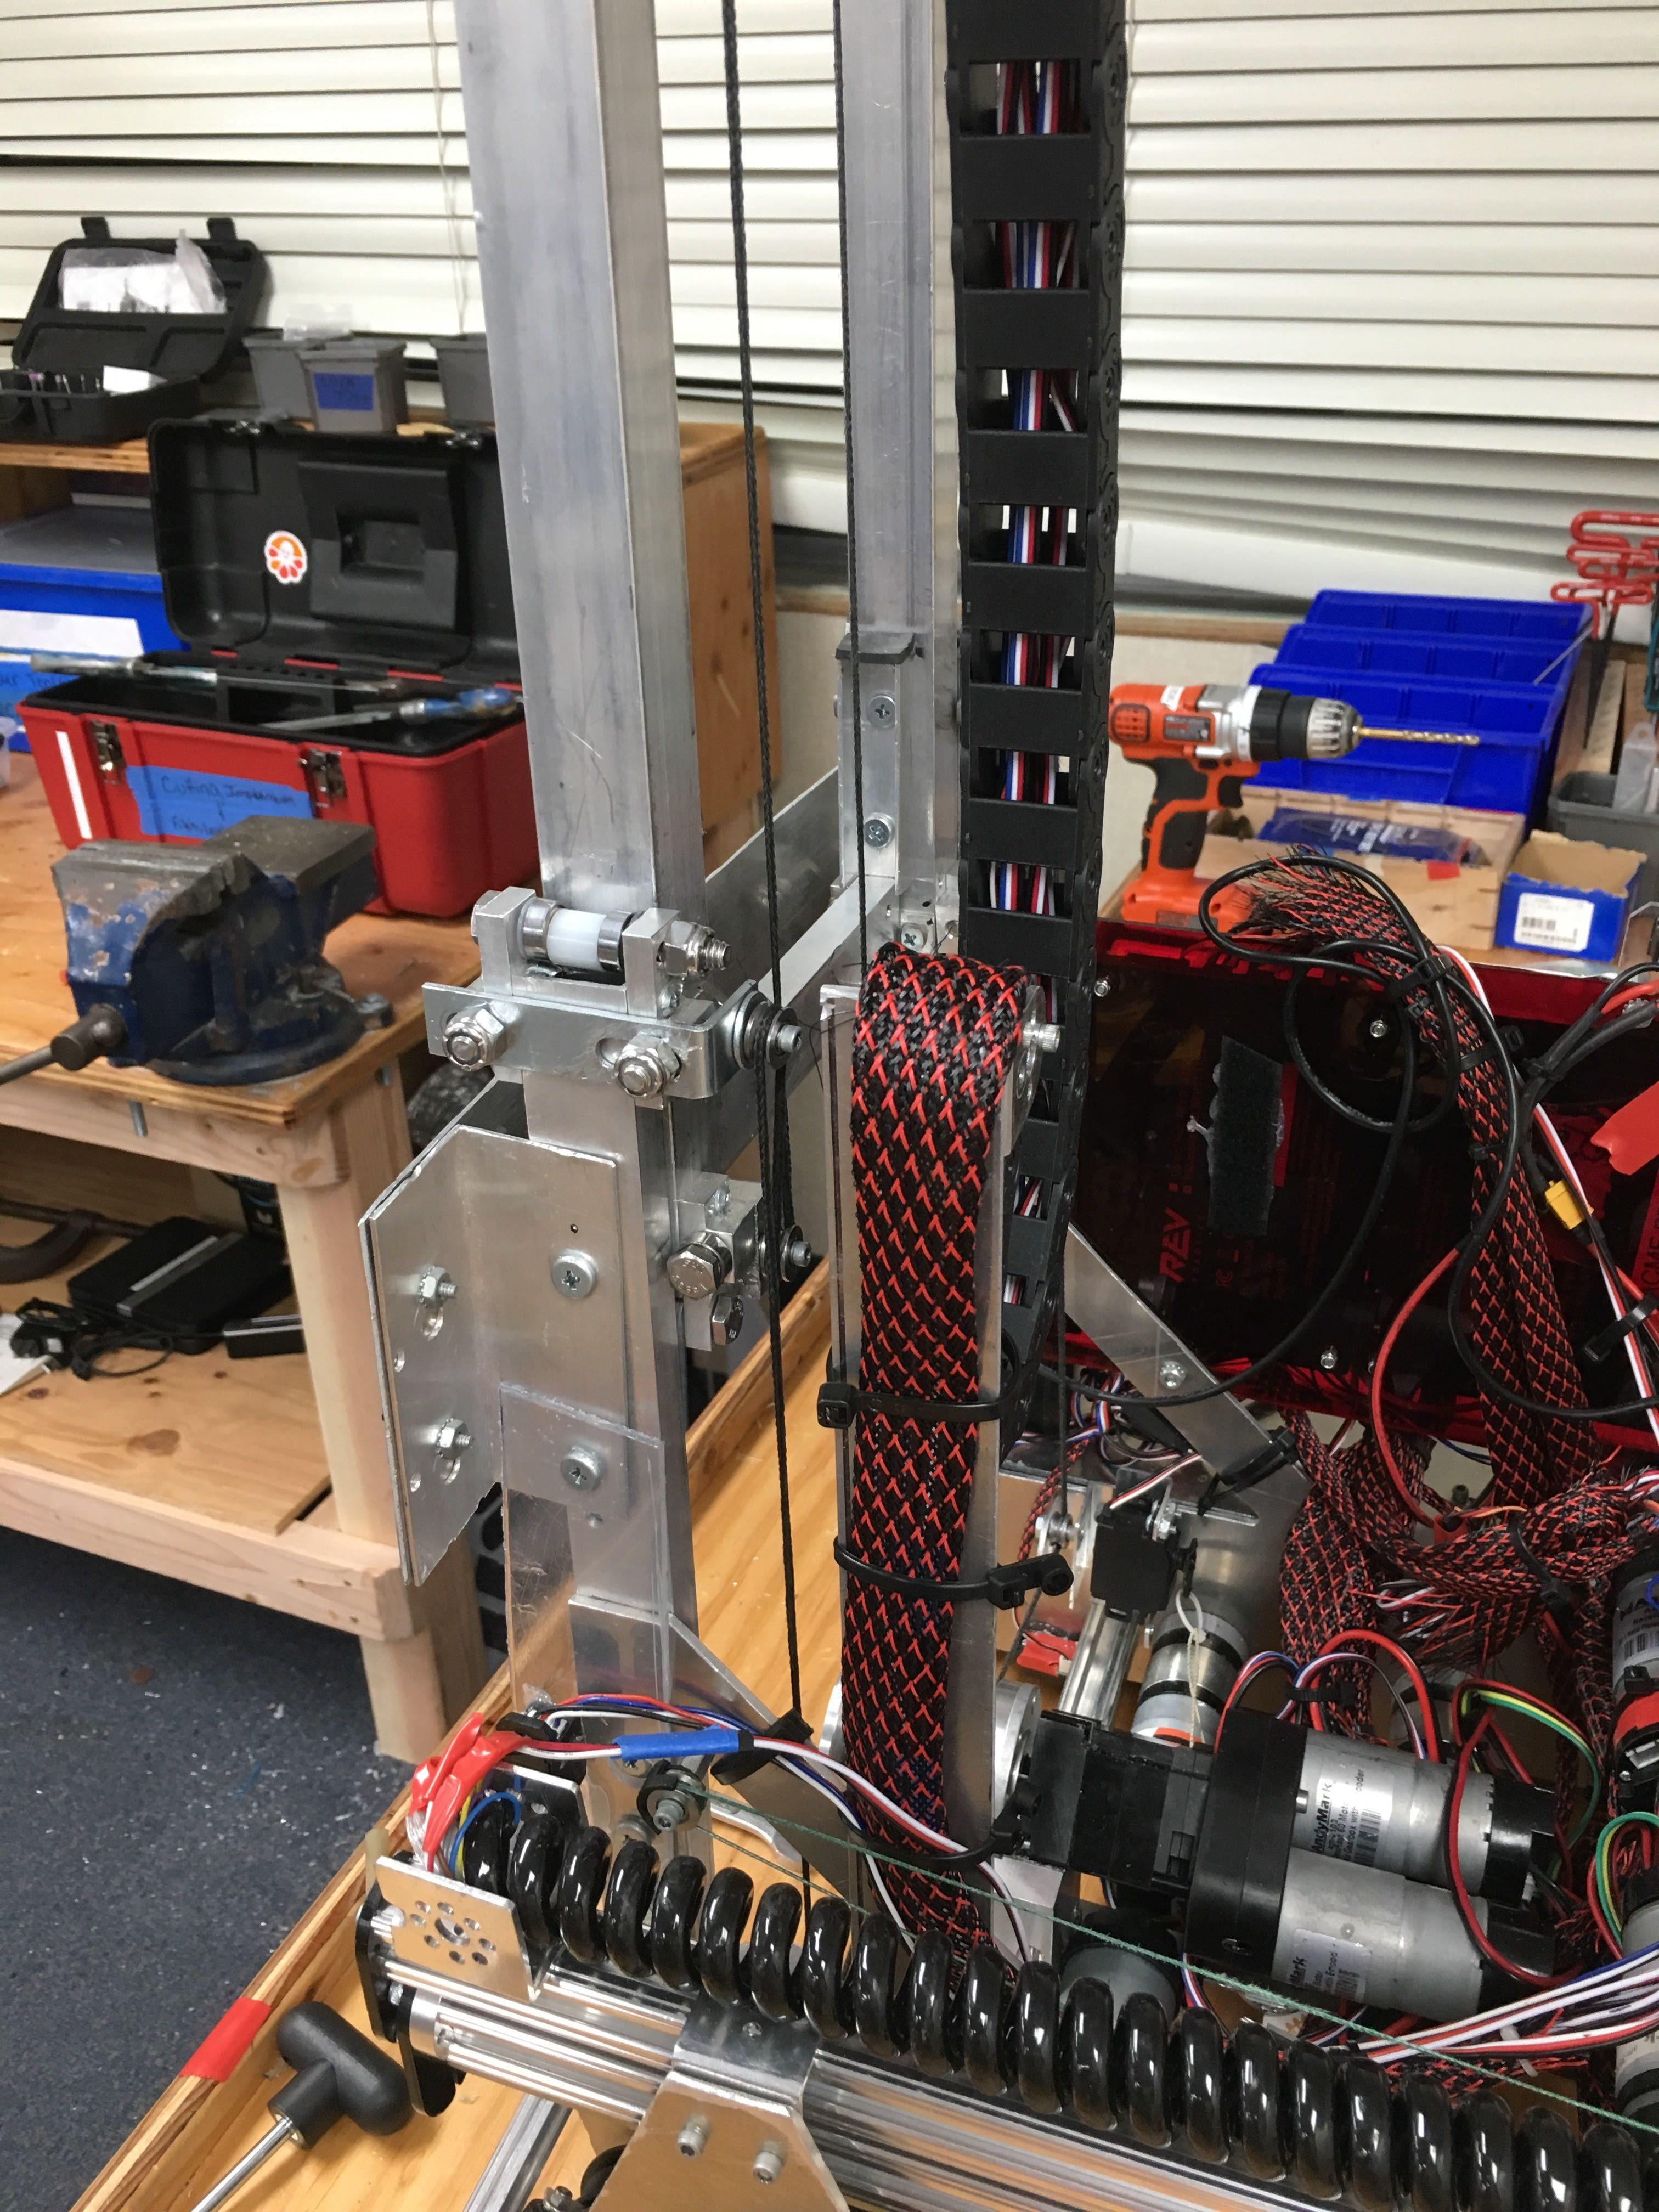
\includegraphics[width= 0.5 \textwidth]{26_02-25/images/PullUpRun2.jpg}
    \caption{New Pull Up Run and Wire Run Up}
    \label{fig:PullUp}
\end{figure}


\subsection{Manufacturing and Installing the New Pull Up Run Standoffs}
Once the CAD drawings were done, Aidan went to GSS to manufacture the parts. He did not complete them in one day because of overlap with Oren fabricating his parts for the lift. Ashlin then went and finished making the parts the next day. He and Aidan then attached them to the lift and made sure that the lift ran smoothly with them. Both parts worked perfectly and did not bend under high levels of stress. Kelly then identified that the bracket standoff also needed to be replaced because it was bending under the stress and flexed. The difficulty with the bracket is that it needed to be positioned to stop rotation on two different axis. Ashlin and Aidan then brainstormed ways to fix this. One idea that was produced was to use a steel bar to reduce this rotation as shown in figure \ref{fig: bracket} Ashlin then went and found the right sized steel and brought it the next meeting. The bracket worked without any bending, which completed the pull up runs as shown in figure \ref{fig: bracket2}.
\begin{figure}
    \centering
    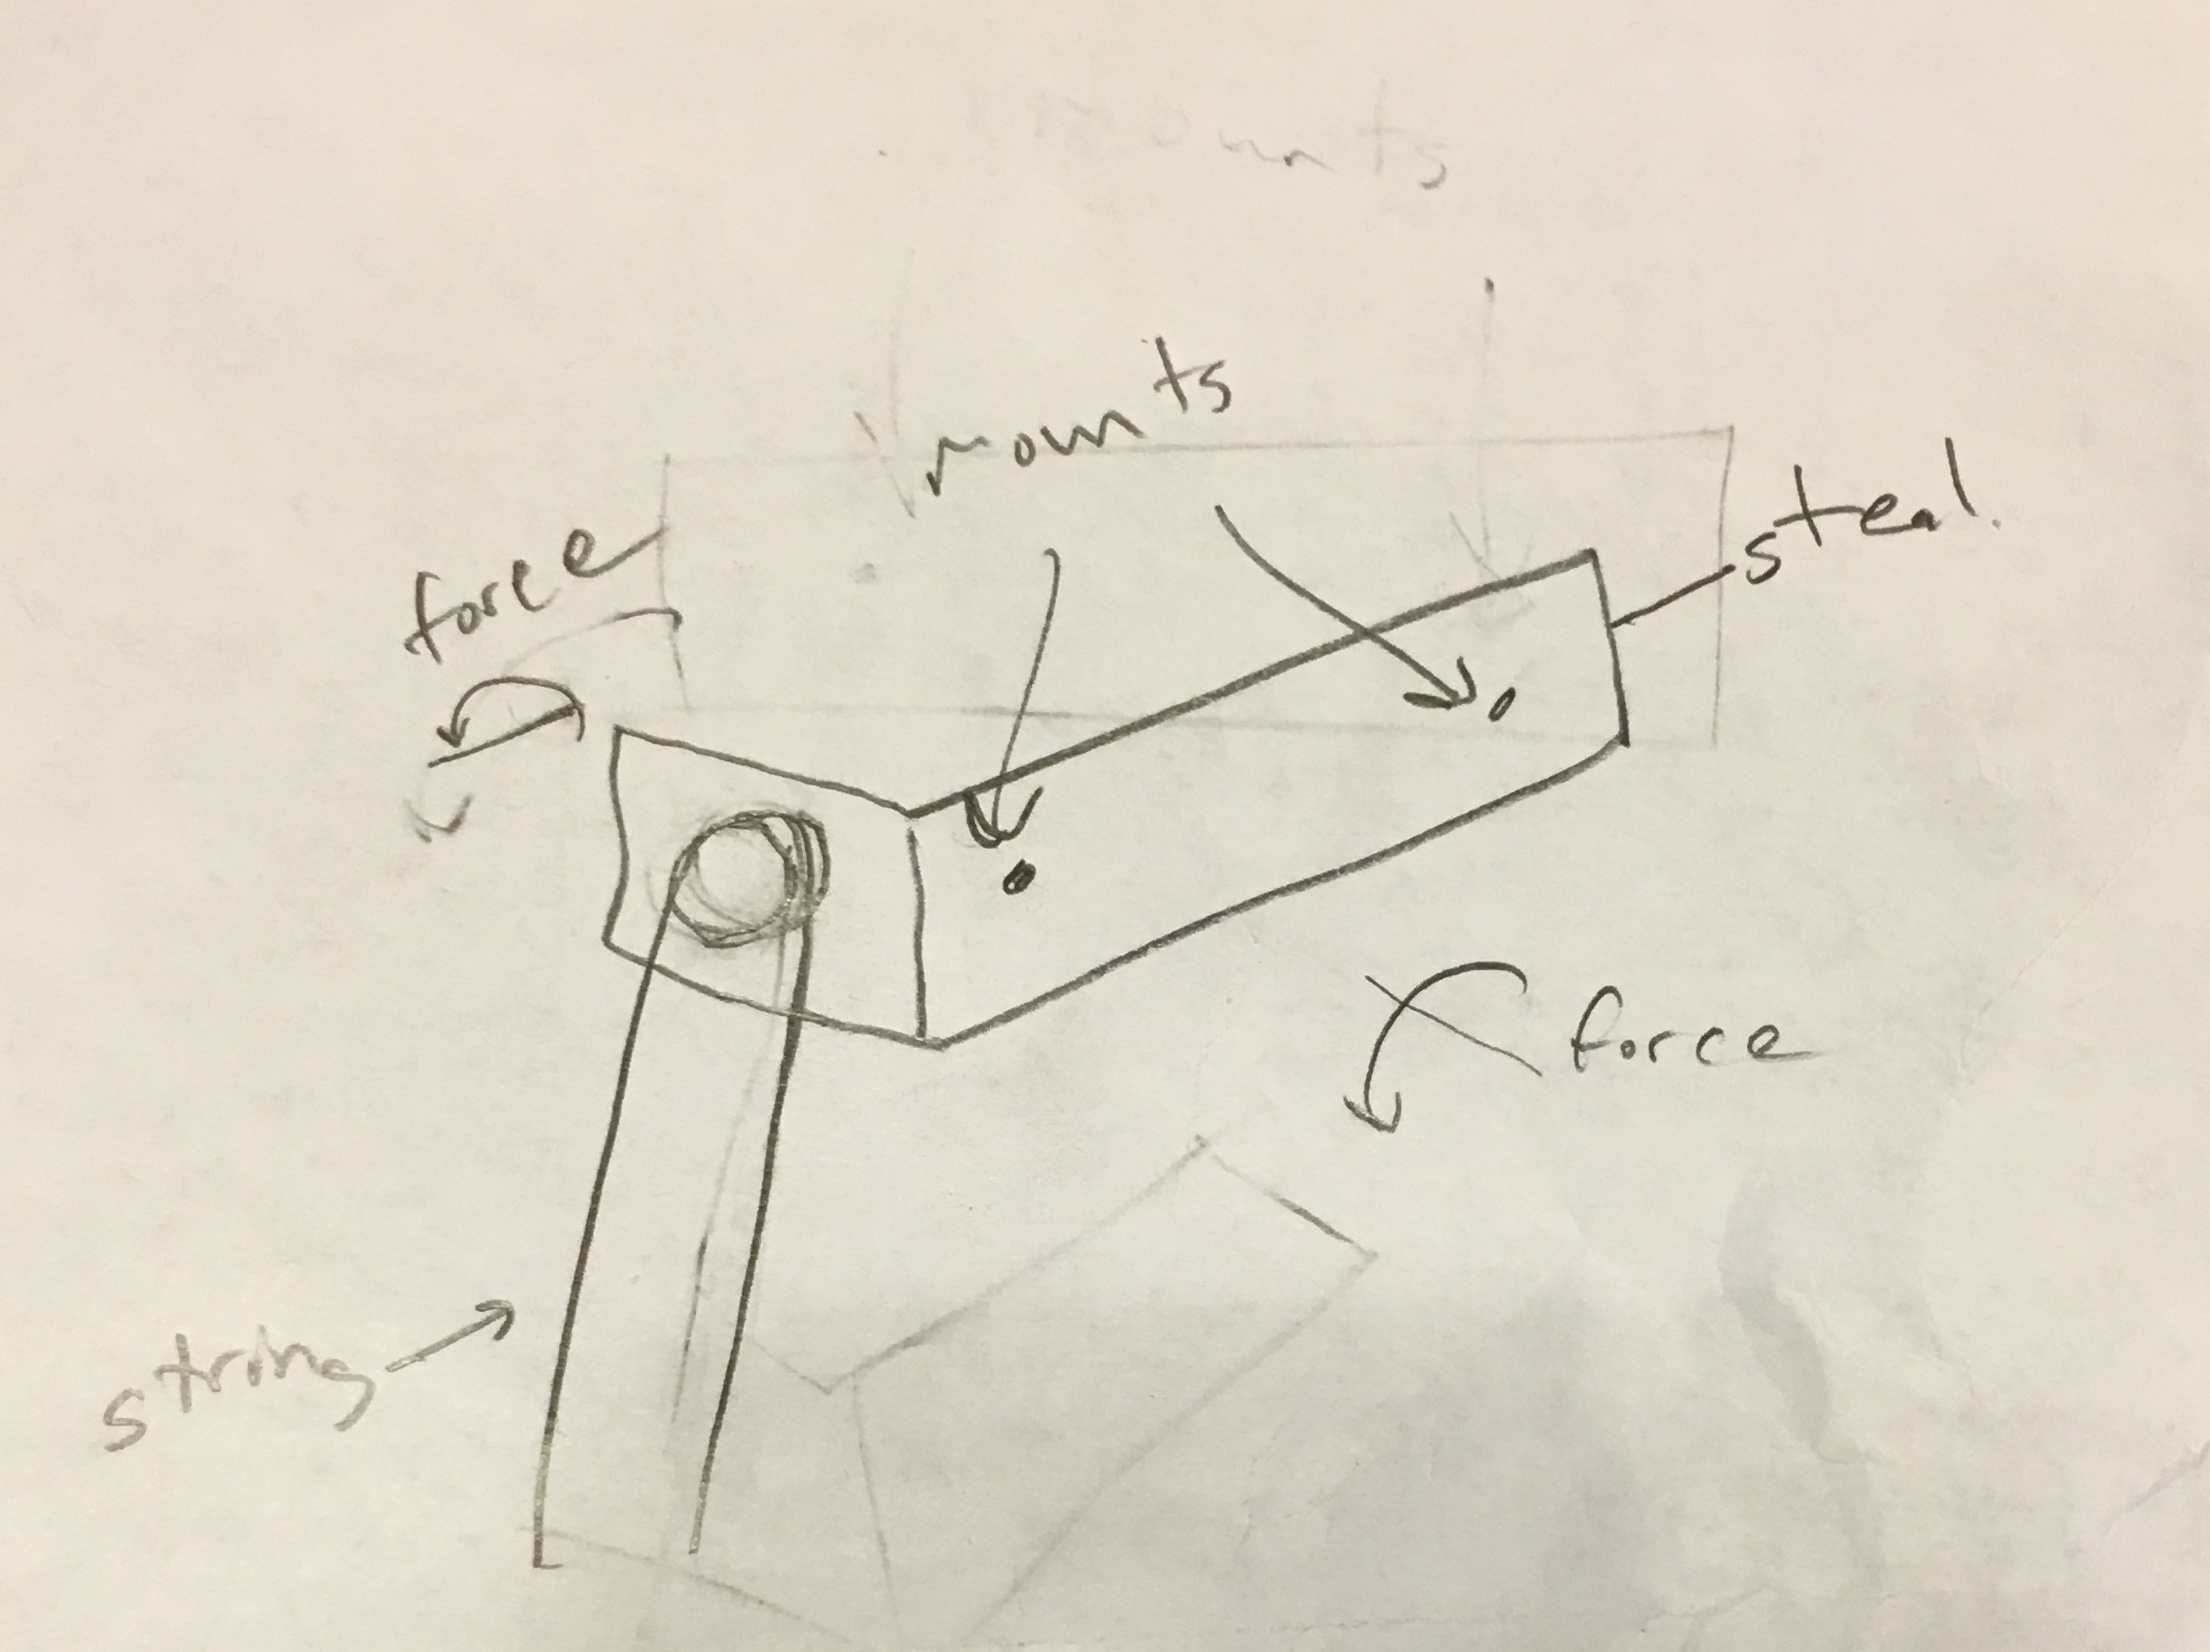
\includegraphics[width= 0.4 \textwidth]{26_02-25/images/Bracket.jpg}
    \caption{Bracket drawing}
    \label{fig: bracket}
\end{figure}
\begin{figure}
    \centering
    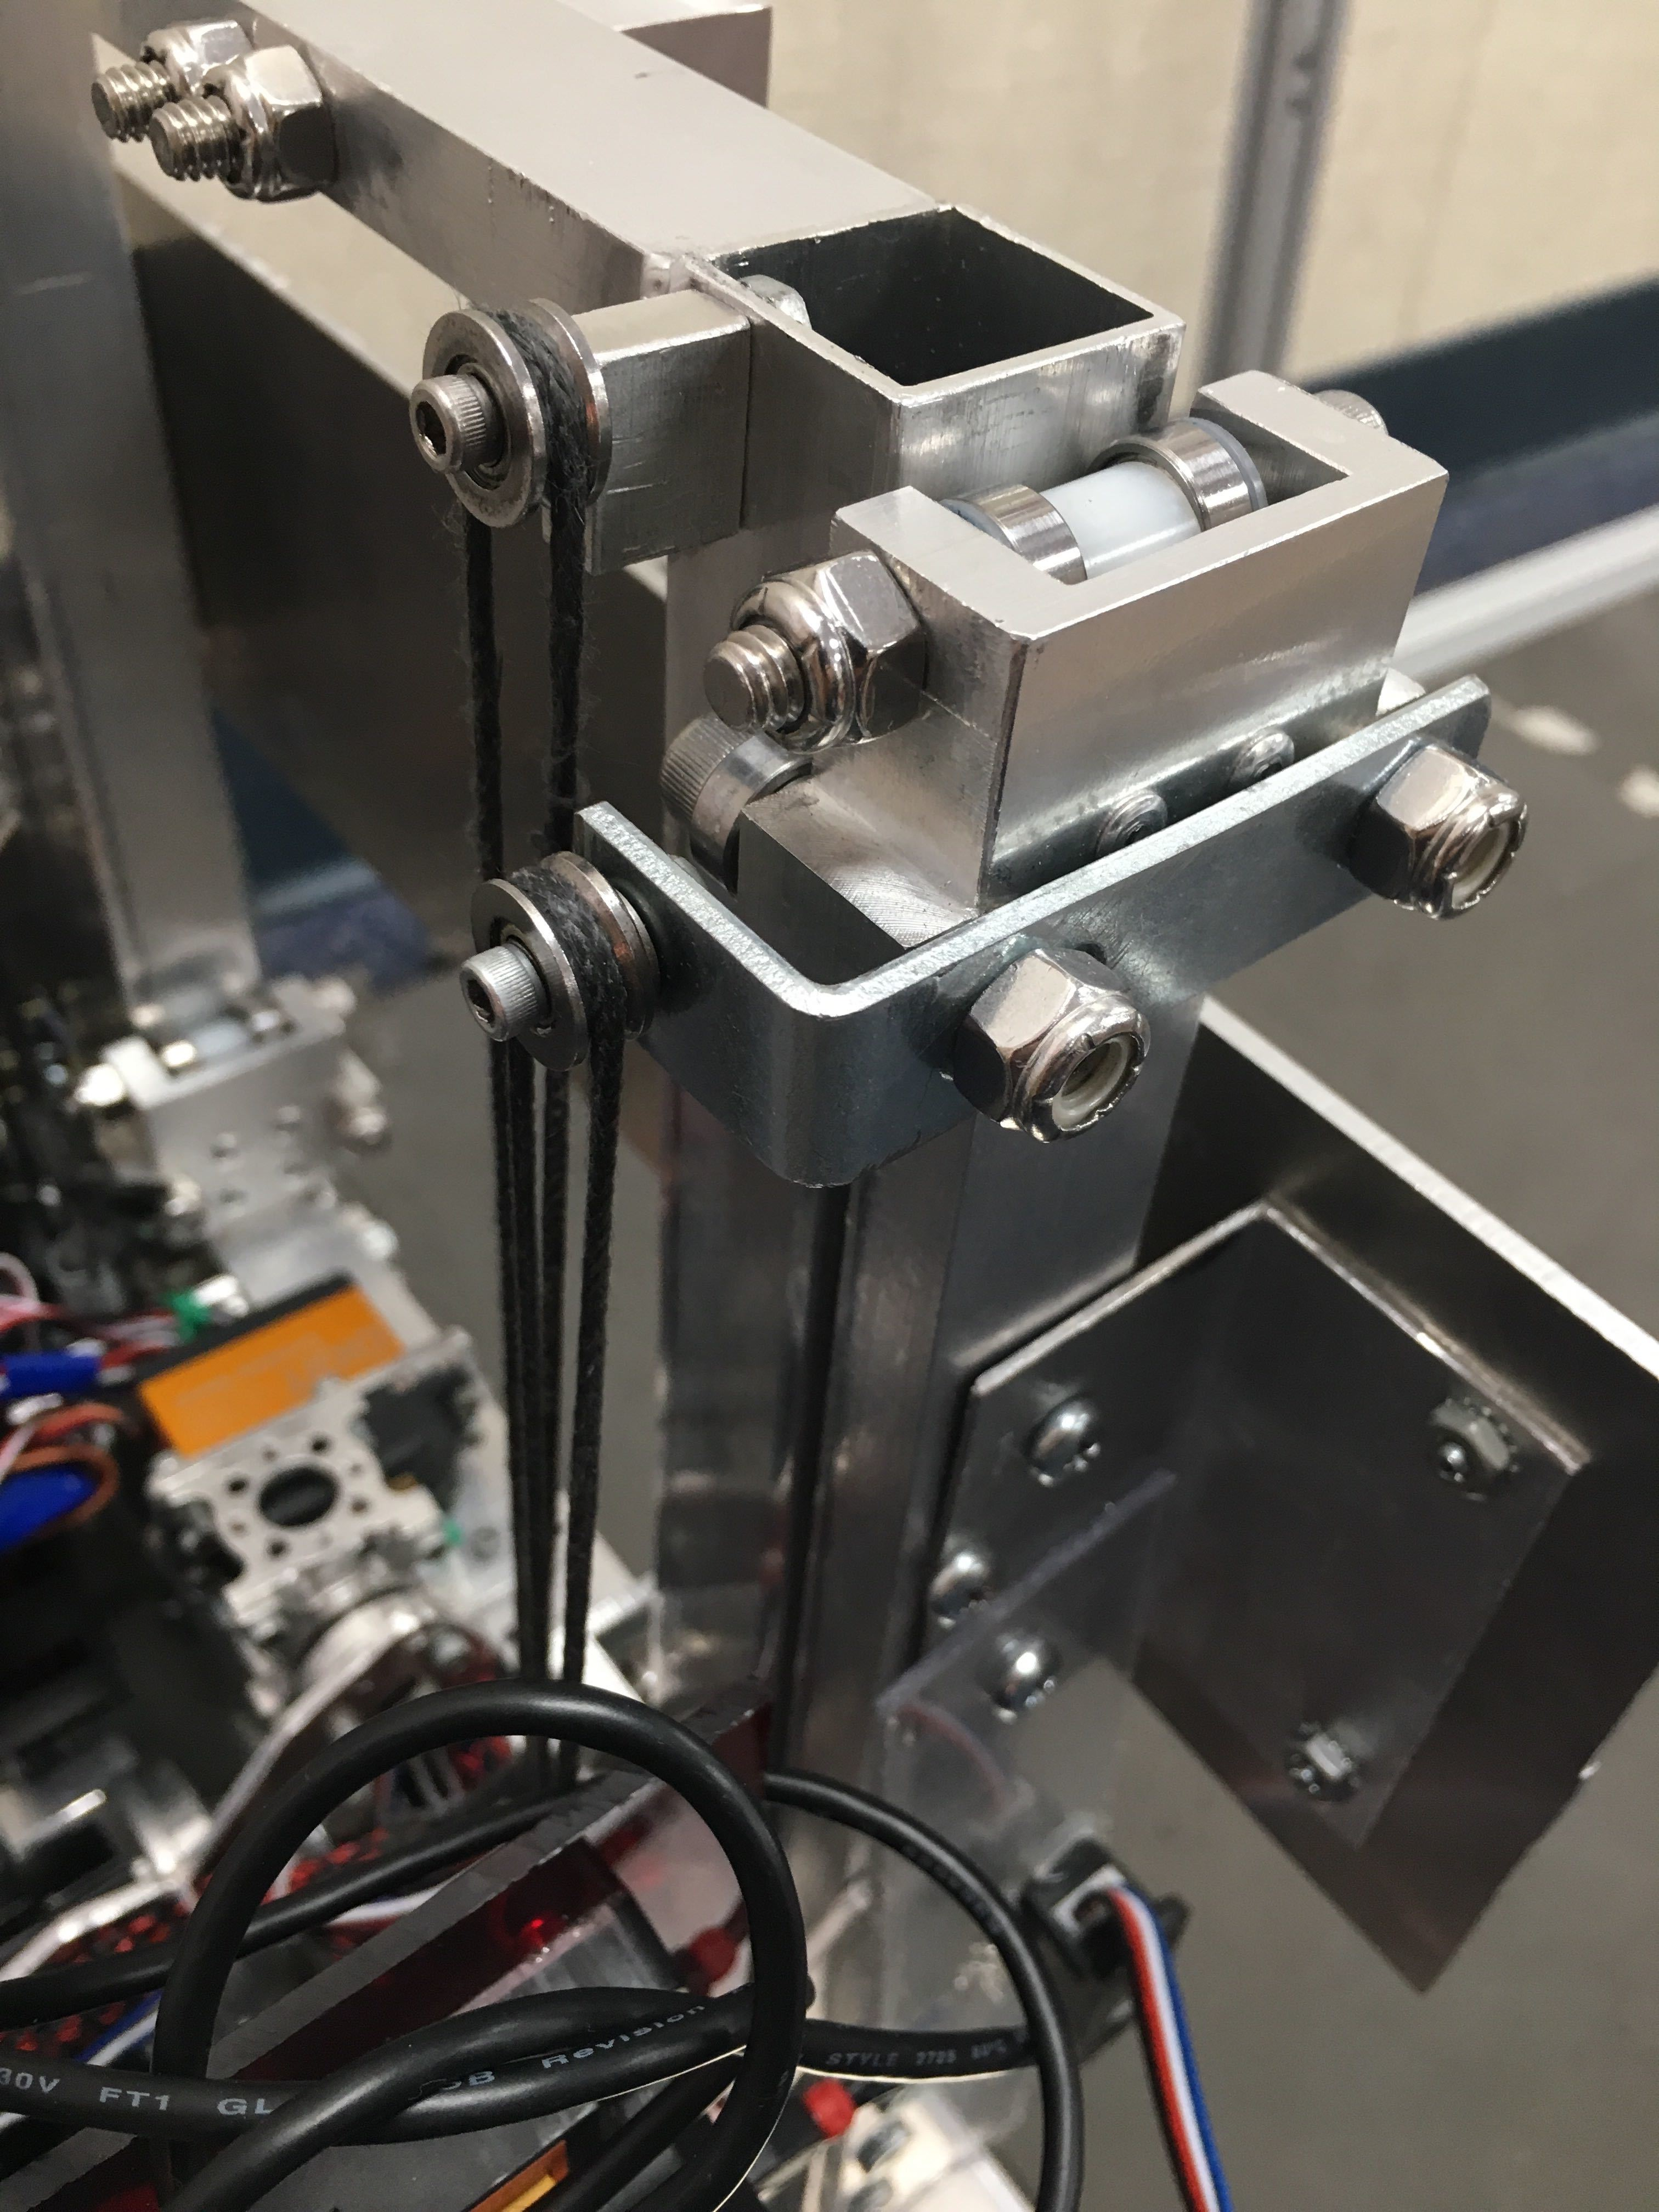
\includegraphics[width= 0.3 \textwidth]{26_02-25/images/Bracket2.jpg}
    \caption{Finished bracket standoff}
    \label{fig: bracket2}
\end{figure}

\end{document}

